\subsection{Integrals in Space}
\subsubsection{Surface Integrals}
Similar to line integrals, a surface integral is an integral evaluated over the surface of a region. It is computed by
$$\iint_S fdS=\iint_S f(\vec{r}(u,v))\|\vec{r}_u\times\vec{r}_v\|dA$$
Note that $dS$ decomposes into $dS=\|\vec{r}_u\times\vec{r}_v\|dA$\\
Ex: Find the surface area of a sphere or radius 2.
\begin{align*}
    &\vec{r}(\theta,\phi)=\brangle{2\cos\theta\sin\phi,2\sin\theta\sin\phi,2\cos\phi}\\
    &\vec{r}_\theta=\brangle{-2\sin\theta\sin\phi,2\cos\theta\sin\phi,0}\\
    &\vec{r}_\phi=\brangle{2\cos\theta\cos\phi,2\sin\theta\cos\phi,-2\sin\phi}\\
    &\vec{r}_\theta\times\vec{r}_\phi=\detmatrix{\hat{i}&\hat{j}&\hat{k}\\-2\sin\theta\sin\phi&2\cos\theta\sin\phi&0\\2\cos\theta\cos\phi&2\sin\theta\cos\phi&-2\sin\phi}\\
    &=\brangle{-4\cos\theta\sin^2\phi,-4\sin\theta\sin^2\phi,-4\sin^2\theta\sin\phi\cos\phi-4\cos^2\theta\sin\phi\cos\phi}\\
    &=\brangle{-4\cos\theta\sin^2\phi,-4\sin\theta\sin^2\phi,-4\sin\phi\cos\phi}\\
    &=-4\sin\phi\brangle{\cos\theta\sin\phi,\sin\theta\sin\phi,\cos\phi}\\
    &\|\vec{r}_\theta\times\vec{r}_\phi\|=4\sin\phi\sqrt{\cos^2\theta\sin^2\phi+\sin^2\theta\sin^2\phi+\cos^2\phi}\\
    &=4\sin\phi\sqrt{\sin^2\phi+\cos^2\phi}\\
    &=4\sin\phi\\
    &\iint_S dS=\int_{\theta=0}^{2\pi}\int_{\phi=0}^{\pi}4\sin\phi=8\pi\brsquare{-\cos\phi}_0^{\pi}=16\pi
\end{align*}
Ex2: Let $S$ be the part of the one-sheeted hyperboloid $x^2+y^2-z^2=1$ which lies above the xy-plane and below the plane $z=A$ where $A$ is a positive constant. Compute the integral $\iint_S zdS$.
\begin{align*}
    &\text{let }\vec{r}(\theta,z)=\brangle{\sqrt{1+z^2}\cos\theta,\sqrt{1+z^2}\sin\theta,z},\ 0\leq\theta\leq 2\pi,\ 0\leq z\leq A\\
    &\vec{r}_\theta=\brangle{-\sqrt{1+z^2}\sin\theta,\sqrt{1+z^2}\cos\theta,0}\\
    &\vec{r}_z=\brangle{\frac{z}{\sqrt{1+z^2}}\cos\theta,\frac{z}{\sqrt{1+z^2}}\sin\theta,1}\\
    &\vec{r}_\theta\times\vec{r}_z=\brangle{\sqrt{1+z^2}\cos\theta,\sqrt{1+z^2}\sin\theta,-z\sin^2\theta-z\cos^2\theta}\\
    &=\brangle{\sqrt{1+z^2}\cos\theta,\sqrt{1+z^2}\sin\theta,-z}\\
    &\|\vec{r}_\theta\times\vec{r}_z\|=\sqrt{(1+z^2)\cos^2\theta+(1+z^2)\sin^2\theta+z^2}=\sqrt{1+z^2+z^2}=\sqrt{1+2z^2}\\
    &\iint_S zdS=\int_{\theta=0}^{2\pi}\int_{z=0}^Az\sqrt{1+2z^2}dzd\theta=2\pi\brsquare{\frac{1}{4}\cdot\frac{2}{3}(1+2z^2)^{3/2}}=\frac{\pi}{3}\brround{(1+2A^2)^{3/2}-1}
\end{align*}
\subsubsection{Flux Integrals}
Integrating a vector field over a surface in $\R^3$ gives a flux integral. This can be thought of how much the vector field is flowing in or out of the surface.\\
Note that a flux integral also requires a choice of orientation. Similar to how a curve had a direction, an orientation states which side of the surface is positive.\\
A flux integral is formed as follows:
$$\iint_S\vec{F}\cdot d\vec{S}=\pm\iint_S\vec{F}\cdot\hat{n} dS=\pm\iint_S\vec{F}(\vec{r}(u,v))\cdot(\vec{r}_u\times\vec{r}_v)dA$$
Ex: Let $S$ be the part of the surface $z=4-x^2-y^2$ lying above the xy-plane, oriented upward. Let $\vec{F}=\brangle{x(x^2+y^2),y(x^2+y^2),z}$. Compute $\iint_S\vec{F}\cdot d\vec{S}$.
\begin{align*}
    &\vec{r}(\theta,z)=\brangle{\sqrt{4-z}\cos\theta,\sqrt{4-z}\sin\theta,z},\ 0\leq\theta\leq 2\pi,\ 0\leq z\leq 4\\
    &\vec{F}(\vec{r})=\brangle{\sqrt{4-z}\cos\theta(4-z),\sqrt{4-z}\sin\theta(4-z),z}\\
    &\vec{r}_z=\brangle{\frac{-1}{2\sqrt{4-z}}\cos\theta,\frac{-1}{2\sqrt{4-z}}\sin\theta,1}\\
    &\vec{r}_\theta=\brangle{-\sqrt{4-z}\sin\theta,\sqrt{4-z}\cos\theta,0}\\
    &\vec{r}_z\times\vec{r}_\theta=\brangle{-\sqrt{4-z}\cos\theta,-\sqrt{4-z}\sin\theta,-\frac{1}{2}(\cos^2\theta+\sin^2\theta)}\\
    &\iint_S\vec{F}\cdot d\vec{S}=-\int_{\theta=0}^{2\pi}\int_{z=0}^4\brround{-(4-z)^2(\cos^2\theta+\sin^2\theta)-\frac{z}{2}}dzd\theta\\
    &=2\pi\brsquare{-\frac{1}{3}(4-z)^3+\frac{z^2}{4}}_0^4\\
    &=2\pi\brround{4+\frac{4^3}{3}}=\frac{152\pi}{3}
\end{align*}
Ex2: Let $S$ be the disk of radius 3, oriented upward on the xy-plane centered at $(15,16,0)$\\
and let $\vec{F}=\brangle{e^{\tan{\sqrt{z}}}+yz,\frac{x\ln(z+1)}{y^6},3+2\cos(z^2)}$.
\begin{align*}
    &\text{note $z=0$ and $x,y>0$ for all points on $S$}\\
    &\vec{F}=\brangle{1,0,5}\\
    &\hat{n}=\hat{k}=\brangle{0,0,1}\\
    &\iint_S\vec{F}\cdot d\vec{S}=\iint_S\brangle{1,0,5}\cdot\brangle{0,0,1}dS=\iint_S5dS=5(9\pi)=45\pi
\end{align*}
\subsubsection{The Divergence Theorem}
Divergence Theorem is given by
$$\oiint_{\partial E}\vec{F}\cdot d\vec{S}=\iiint_E(\nabla\cdot \vec{F})dV$$
where $E$ is a solid region in $\R^3$ and $\partial E$ is the boundary of $E$ oriented outward.\\
This formula can be thought of as the rate that fluid escapes $E$ is equal to the total rate of fluid being produced.\\
Ex: Find the flux from the vector field $\vec{F}=\brangle{x,y,z}$ out of the cube of side length 2 centered at the origin.
\begin{align*}
    &\nabla\cdot \vec{F}=3\\
    &\iiint_E 3dV=3\cdot\text{Vol}(E)=24
\end{align*}
Ex2: Let $S$ be the hemisphere of radius 1 located above the xy-plane, oriented outward\\
and let $\vec{F}=\brangle{z^2x,\frac{1}{3}y^3+\tan\sqrt{z},x^2z+y^2}$. Find $\iint_S\vec{F}\cdot d\vec{S}$.\\
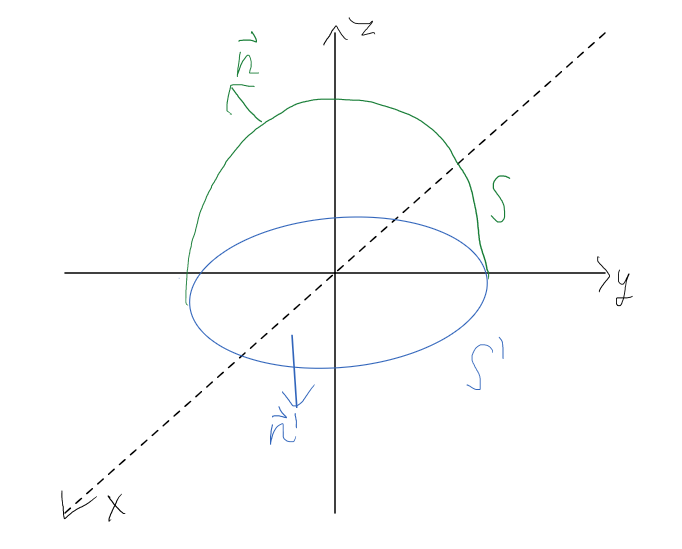
\includegraphics[scale=0.5]{Images/Math217Pictures/divergenceThmEx.png}
\begin{align*}
    &\nabla\cdot \vec{F}=z^2+y^2+x^2=\rho^2\\
    &\partial E=S+S'\\
    &E=\brcurly{x^2+y^2+z^2\leq1,\ z\geq0}\\
    &S'=\brcurly{x^2+y^2=1\ z=0}\\
    &\iiint_E \rho^2dV=\iint_S\vec{F}\cdot d\vec{S}+\iint_{S'}\vec{F}\cdot d\vec{S}\\
    &\iiint_E\rho^2dV=\int_{\theta=0}^{2\pi}\int_{\phi=0}^{\pi/2}\int_{\rho=0}^1\rho^4\sin\phi d\rho d\phi d\theta=2\pi\brsquare{-\cos\phi}_0^{\pi/2}\brsquare{\frac{\rho^5}{5}}_0^1=\frac{2\pi}{5}\\
    &\iint_{S'}\vec{F}\cdot d\vec{S}=\brangle{z^2x,\frac{1}{3}y^3+\tan\sqrt{z},x^2z+y^2}\cdot\brangle{0,0,-1}dS=-\iint_{S'}x^2z+y^2 dS\\
    &\iint_{S'}\vec{F}\cdot d\vec{S}=-\iint_{S'}y^2dS=-\int_{\theta=0}^{2\pi}\int_{r=0}^1r^3\sin^2\theta drd\theta=-\pi\brsquare{\frac{r^4}{4}}_0^1=-\frac{\pi}{4}\\
    &\iint_S\vec{F}\cdot d\vec{S}=\iiint_E\rho^2dV-\iint_{S'}\vec{F}\cdot d\vec{S}=\frac{5\pi}{2}+\frac{\pi}{4}=\frac{13\pi}{20}
\end{align*}
It is also important to note that to apply the divergence theorem, the vector field must be defined within the region.\\
Ex3: Find the flux from the vector field $\vec{F}=\frac{\vec{r}}{r^3}$ out of the surface $\partial E$ where $E$ is the sphere of radius 2 centered about the origin.\\
Note that because the vector field is undefined at the origin, we need to compute the flux about the origin separately.\\
We can define the sphere $S_{\epsilon}$ to be the sphere of radius $\epsilon$ about the origin for where $\epsilon\to0$ and subtract its flux from the total flux of the region.\\
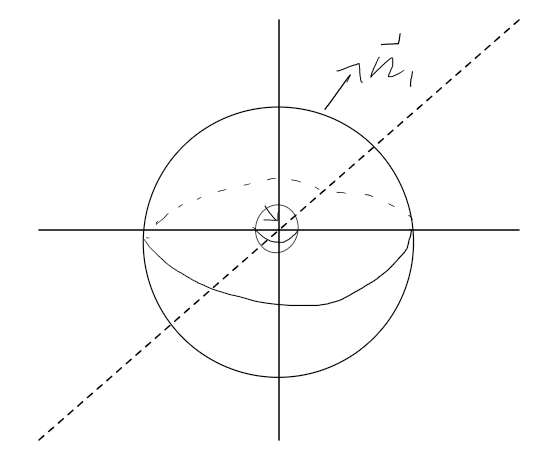
\includegraphics[scale=0.5]{Images/Math217Pictures/divergenceThmEx2.png}
\begin{align*}
    &\iiint_{\partial E}(\nabla\cdot \vec{F})dV=\iint_S\vec{F}\cdot d\vec{S}+\iint_{S_{\epsilon}}\vec{F}\cdot d\vec{S}\\
    &\vec{F}=\brangle{\frac{x}{(x^2+y^2+z^2)^{3/2}},\frac{y}{(x^2+y^2+z^2)^{3/2}},\frac{z}{(x^2+y^2+z^2)^{3/2}}}\\
    &\nabla\cdot\vec{F}=0\\
    &\hat{n}_2=-\frac{\vec{r}}{r}\\
    &\iint_{S_{\epsilon}}\vec{F}\cdot d\vec{S}=\iint_{S_{\epsilon}}\frac{\vec{r}}{r^3}\cdot\frac{-\vec{r}}{r}dS=-\iint_{S_{\epsilon}}\frac{1}{r^2}dS=-\frac{1}{\epsilon^2}\iint_{S_{\epsilon}}dS=-\frac{1}{\epsilon^2}\cdot 4\pi\epsilon^2=-4\pi\\
    &\iint_S\vec{F}\cdot d\vec{S}=-\iint_{S_{\epsilon}}\vec{F}\cdot d\vec{S}=4\pi
\end{align*}
\subsubsection{Stokes' Theorem}
Stokes' Theorem is a more general case of Green's Theorem and is given by
$$\oint_{\partial S}\vec{F}\cdot d\vec{r}=\iint_S(\nabla\times\vec{F})\cdot d\vec{S}$$
Ex: Compute $\oint_C\vec{F}\cdot d\vec{r}$ where $C$ is given by $\vec{r}(t)=\brangle{\sin t,\cos t,-\sin 2t}$\\
and $\vec{F}=\brangle{\tan\sqrt{1+x^4},zy+e^{y^3},\frac{x^2}{2}+\sqrt[3]{\sin(z^2)}}$\\
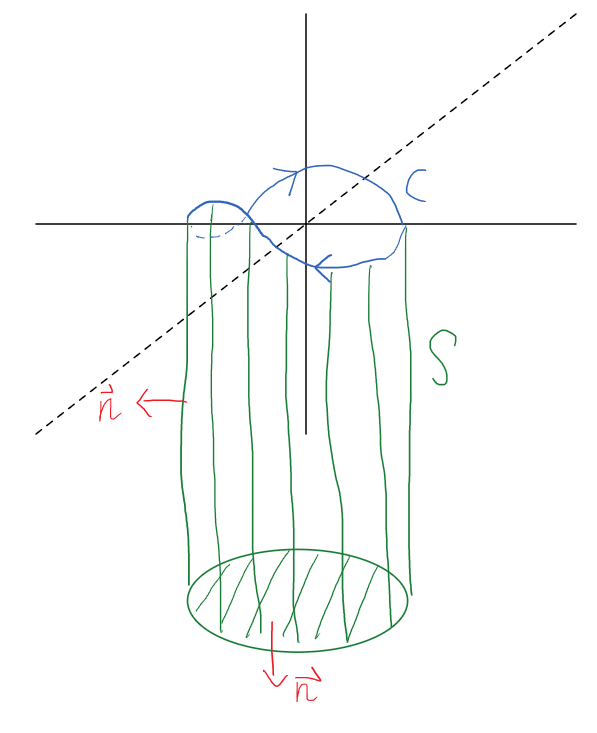
\includegraphics[scale=0.5]{Images/Math217Pictures/stokesThmEx.png}
\begin{align*}
    &\nabla\times\vec{F}=\brangle{-y,-x,0}\\
    &S_1=\brcurly{x^2+y^2=1}\\
    &S_2=\brcurly{z=-A}\\
    &\oint\vec{F}\cdot d\vec{r}=\iint_{S_1}(\nabla\times\vec{F})
    cdot d\vec{S}+\iint_{S_2}(\nabla\times\vec{F})\cdot d\vec{S}\\
    &\iint_{S_2}\brangle{-y,-x,0}\cdot\brangle{0,0,-1}dS=0\\
    &S_1:\ \vec{r}(\theta,z)=\brangle{\cos\theta,\sin\theta,z},\ 0\leq \theta\leq 2\pi,\ -A\leq z\leq -\sin 2\theta\\
    &\vec{r}_z=\brangle{0,0,1}\\
    &\vec{r}_\theta=\brangle{-\sin\theta,\cos\theta,0}\\
    &\vec{r}_z\times\vec{r}_\theta=\brangle{-\cos\theta,-\sin\theta,0}\\
    &\iint_{S_1}(\nabla\times\vec{F})\cdot d\vec{S}=-\int_{\theta=0}^{2\pi}\int_{z=-A}^{-\sin 2\theta}\brangle{-\sin\theta,-\cos\theta,0}\cdot\brangle{-\cos\theta,-\sin\theta,0}dzd\theta\\
    &=\int_0^{2\pi}\int_{-A}^{-\sin2\theta}-2\sin\theta\cos\theta dzd\theta=\int_0^{2\pi}-2\sin\theta\cos\theta\brround{-\sin2\theta+A}d\theta\\
    &=\int_0^{2\pi}(\sin^2(2\theta)-A\sin(2\theta))d\theta=\pi\\
    &\Ra\oint\vec{F}\cdot d\vec{r}=\pi
\end{align*}
\subsubsection{Differential Forms}
Differential forms are the unifying language of derivatives and integrals.\\
Let $x_1,\ldots,x_n$ be coordinates on $\R^n$. We can introduce the \textit{wedge product} such that $dx_i\wedge dx_j=-dx_j\wedge dx_i$. Now let $U\subset\R^n$ be an open set. A differential k-form is a linear combination of k-fold products of $dx$'s with functions on $U$ as coefficients.\\
For example, a 1-form corresponds to $Pdx+Qdy+Rdz$ and a 2-form can be written as $Pdy\wedge dz+Qdz\wedge dx+Rdx\wedge dy$\\
Notice that with wedge products there is also the rule $dx\wedge dx=0$.\\
Zero forms are just functions.\\
A set of k-forms are written as $\Omega^k(U)$.\\
\begin{tabular}{c|c|c}
    $k$-form & expression & geometric meaning\\
    \hline
    $\Omega^0(U)$ & $f$ & function\\
    $\Omega^1(U)$ & $F_1dx+F_2dy+F_3dz$ & vector field\\
    $\Omega^2(U)$ & $F_1dy\wedge dz+F_2dz\wedge dx+F_3dx\wedge dy$ & vector field\\
    $\Omega^3(U)$ & $fdx\wedge dy\wedge dz$ & function
\end{tabular}\\
A wedge product is computed as 
$$\Omega^k(U)\wedge\Omega^l(U)\to\Omega^{k+l}(U)$$
This allows us to express vector operations in terms of wedge products in a more compact notation.\\
Ex: The cross product is given by $\Omega^1(U)\wedge\Omega^1(U)\to\Omega^2(U)$
\begin{align*}
    &F,G\in\Omega^1(\R^3)\\
    &F\wedge G=(F_1dx+F_2dy+F_3dz)\wedge(G_1dx+G_2dy+G_3dz)\\
    &=F_1G_2dx\wedge dy+F_1G_3dx\wedge dz+F_2G_1dy\wedge dx+F_2G_3dy\wedge dz+F_3G_1dz\wedge dx+F_3G_2dz\wedge dy\\
    &=(F_2G_3-F_3G_2)dy\wedge dz+(F_3G_1-F_1G_3)dz\wedge dx+(F_1G_2-F_2G_1)dx\wedge dy\\
    &=\vec{F}\times\vec{G}
\end{align*}
Ex2: The dot product is given by $\Omega^1(U)\wedge\Omega^2(U)\to\Omega^3(U)$
\begin{align*}
    &F\in\Omega^1(\R^3)\\
    &G\in\Omega^2(\R^3)\\
    &F\wedge G=(F_1dx+F_2dy+F_3dz)\wedge(G_1dy\wedge dz+G_2dz\wedge dx+G_3dx\wedge dy)\\
    &=F_1G_1dx\wedge dy\wedge dz+F_2G_2 dy\wedge dz\wedge dx+F_3G_3 dz\wedge dx\wedge dy\\
    &=(F_1G_1+F_2G_2+F_3G_3)dx\wedge dy\wedge dz\\
    &=\vec{F}\cdot \vec{G}
\end{align*}
Differential forms also allows us to generalize the types of derivatives (gradient, curl, divergence) into one derivative.
$$d\Omega^k(U)\to\Omega^{k+1}(U)$$
\begin{tabular}{c|c|c}
    $\Omega^k(U)$ & derivative transformation & Type of derivative\\
    \hline
    $\Omega^0(U)$ & scalar to vector field & gradient ($\nabla f$)\\
    $\Omega^1(U)$ & vector field to vector field & curl ($\nabla\times \vec{F}$)\\
    $\Omega^2(U)$ & vector field to scalar & divergence ($\nabla\cdot\vec{F}$)
\end{tabular}\\
In general, taking a derivative twice gives 0. $d(d\Omega^k(U))=0$\\
Differential forms also allows us to easily define product rules using the following formula.\\
If $\alpha\in\Omega^k(U)$ and $\beta\in\Omega^l(U)$ then
$$d(\alpha\wedge\beta)=d\alpha\wedge\beta+(-1)^k\alpha\wedge d\beta$$
\begin{align*}
    \text{Ex: }&\nabla\times(f\vec{F})\\
    &f\in\Omega^0(U),\ \vec{F}\in\Omega^1(U)\\
    &\nabla\times(f\vec{F})=\nabla f\times\vec{F}+f(\nabla\times\vec{F})
\end{align*}
\begin{align*}
    \text{Ex2: }&\nabla\cdot(\vec{A}\times\vec{B})\\
    &\vec{A},\vec{B}\in\Omega^1(U)\\
    &\nabla\cdot(\vec{A}\times\vec{B})=(\nabla\times\vec{A})\cdot\vec{B}-\vec{A}\cdot(\nabla\times\vec{B})
\end{align*}
Similar to derivatives, we can go in the opposite direction and generalize multiple integration using differential forms.\\
If $M$ is a (k+1)-manifold, $\partial M$ is a k-manifold, $\alpha$ is a k-form, and $d\alpha$ is a (k+1)-form then we can write the generalized Stokes' Theorem as
$$\int_{\partial M}\alpha=\int_M d\alpha$$
Differential forms also behave nicely under a change of variables.
\begin{align*}
    \text{Ex: }&\eqnsystem{x=r\cos\theta\\y=r\sin\theta}\\
    &dx=\frac{\partial x}{\partial r}dr+\frac{\partial x}{\partial \theta}d\theta=\cos\theta dr-r\sin\theta d\theta\\
    &dy=\frac{\partial y}{\partial r}dr+\frac{\partial y}{\partial\theta}d\theta=\sin\theta dr+r\cos\theta d\theta\\
    &dx\wedge dy=(\cos\theta dr-r\sin\theta d\theta)\wedge(\sin\theta dr+r\cos\theta d\theta)\\
    &=r\cos^2\theta dr\wedge d\theta+r\sin^2\theta dr\wedge d\theta=rdr\wedge d\theta
\end{align*}